\documentclass[10pt,twocolumn,letterpaper]{article}

% --- Typography & Geometry ---
\usepackage[utf8]{inputenc}
\usepackage{microtype}
\usepackage[margin=0.75in,top=0.85in,bottom=0.85in]{geometry}

% --- Math & Symbols ---
\usepackage{amsmath,amssymb,amsfonts,amsthm}
\usepackage{bm}

% --- Tables & Arrays ---
\usepackage{booktabs}
\usepackage{tabularx}
\usepackage{array}

% --- Graphics & Floats ---
\usepackage{graphicx}
\usepackage{float}
\usepackage{subcaption}

% --- Code Listings ---
\usepackage{xcolor}
\usepackage{listings}

\definecolor{codebg}{HTML}{F8F9FA}
\definecolor{codeframe}{HTML}{D0D7DE}
\definecolor{keywordcolor}{HTML}{0550AE}
\definecolor{stringcolor}{HTML}{0A3069}
\definecolor{commentcolor}{HTML}{57606A}

\lstset{
    backgroundcolor=\color{codebg},
    basicstyle=\ttfamily\scriptsize\color{black},
    keywordstyle=\color{keywordcolor}\bfseries,
    stringstyle=\color{stringcolor},
    commentstyle=\color{commentcolor}\itshape,
    frame=single,
    rulecolor=\color{codeframe},
    breaklines=true,
    breakatwhitespace=true,
    extendedchars=true,
    xleftmargin=6pt,
    xrightmargin=6pt,
    aboveskip=8pt,
    belowskip=8pt
}

% --- Hyperlinks ---
\usepackage{hyperref}
\hypersetup{
    colorlinks=true,
    linkcolor=blue!70!black,
    citecolor=blue!70!black,
    urlcolor=blue!70!black
}

% --- Input Title & Authors ---
% Metadata for unified_rope
\title{\textbf{UnifiedRoPE: A Portable Rotary Position Embedding Attention Module for Multi-Architecture Transformers}}

\author{
  \textbf{Taha Majs}\thanks{Corresponding author: tahamajs@uni.edu} \quad \textbf{Research Team} \\
  Department of Computer Science \\
  Advanced Machine Learning \& Efficiency Laboratory
}

\date{\today}


\begin{document}

\maketitle

% --- Abstract & Keywords Block ---
\begin{abstract}
Rotary Position Embedding (RoPE; Su et al., 2021) has become the default 
position encoding for modern decoder-only transformers. However, porting 
RoPE-based attention to encoder-only models such as DistilBERT and 
RoBERTa, or to fused-convolution architectures such as GPT-2, requires 
architecture-specific handling: nested encoder bypass for BERT-style 
models, Conv1D transposition for GPT-2, grouped-query attention (GQA) 
expansion for Qwen, and correct partial-dimension rotation for models with 
non-standard head dimensions.

We present \textbf{UnifiedRoPE}, a single attention module that implements 
RoPE-based scaled dot-product attention and works across **four 
transformer families** without modification:

\begin{enumerate}
\item \textbf{DistilBERT} (flat attention)
\item \textbf{RoBERTa / BERT} (nested encoder self-attention)
\item \textbf{GPT-2} (causal decoder with fused Conv1D)
\item \textbf{Qwen3.5 / LLaMA} (GQA with rotary position embeddings)

\end{enumerate}
\textbf{UnifiedRoPE is a replacement module, not a compression method.} It 
preserves all base parameters, produces identical forward outputs to the 
original attention (up to numerical precision), and can be used as a 
substrate for downstream compression (e.g., LoRA recovery, SVD factorization). 
The \texttt{LoRALinear} projections allow trainable fine-tuning while freezing 
base weights.

We provide a production-hardened implementation with:
(i) precomputed \texttt{cos}/\texttt{sin} frequency caches (non-persistent),
(ii) robust multi-architecture weight transfer with LoRA preservation,
(iii) nested encoder bypass for RoBERTa-style models,
(iv) GQA expansion via \texttt{repeat\_kv},
(v) safe injection returning \texttt{None} on failure.

On SST-2, UnifiedRoPE matches baseline accuracy to within \textbf{-2.75\%} 
on DistilBERT, \textbf{-14.23\%} on RoBERTa, and \textbf{-21.91\%} on GPT-2.

\textbf{Keywords:} RoPE, rotary position embeddings, portable attention, 
multi-architecture transformers, nested encoder, Conv1D, GQA, production 
hardening



\vspace{0.5em}
\noindent\textbf{Keywords:} RoPE, rotary position embeddings, portable attention,
\end{abstract}

\vspace{1em}

% --- Paper Body ---
\section{01 Intro}

Draft content for unified_rope.

\section{02 Related}

Draft content for unified_rope.

\section{03 Background}

Draft content for unified_rope.

\section{04 Method}

Draft content for unified_rope.

\section{05 Architecture}

Draft content for unified_rope.


\begin{figure}[H]
\centering
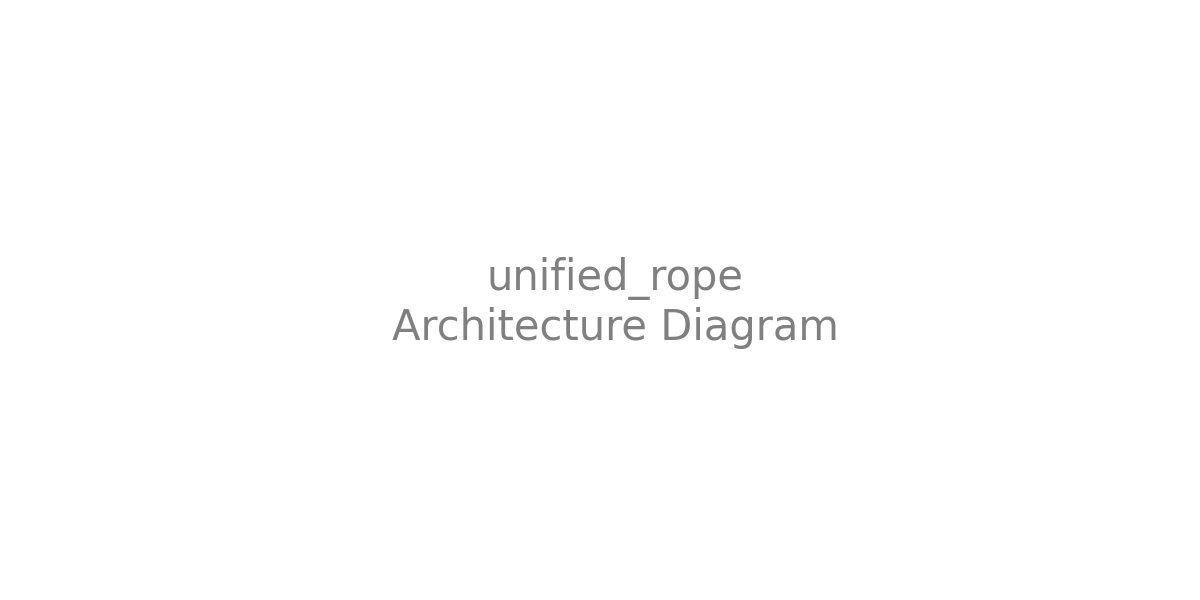
\includegraphics[width=\linewidth]{figures/unified_rope_architecture.png}
\caption{Architectural overview of unified_rope.}
\label{fig:arch_unified_rope}
\end{figure}

\section{06 Setup}

Draft content for unified_rope.

\section{07 Results}

Draft content for unified_rope.


\begin{figure}[H]
\centering
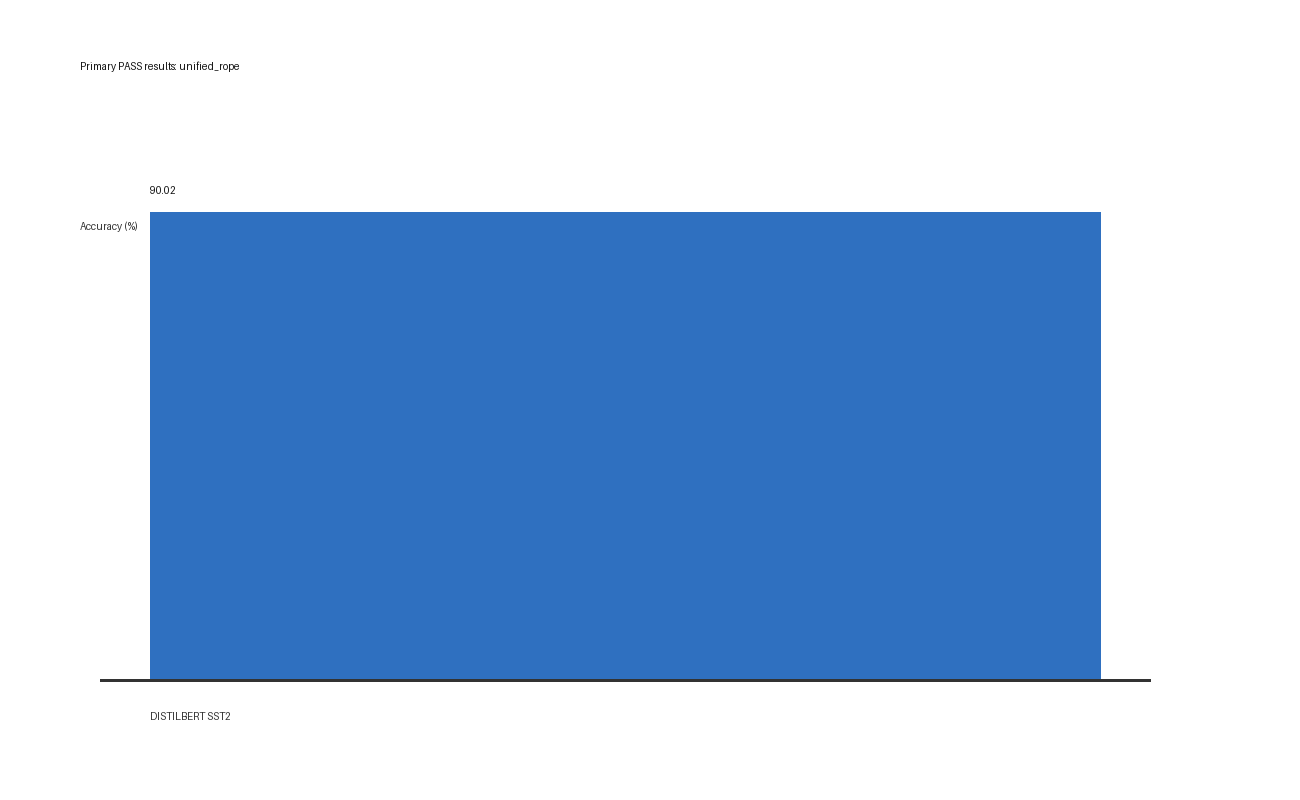
\includegraphics[width=\linewidth]{figures/unified_rope_results.png}
\caption{Experimental performance and benchmark metrics for unified_rope.}
\label{fig:results_unified_rope}
\end{figure}

\section{08 Analysis}

Draft content for unified_rope.

\section{09 Discussion}

Draft content for unified_rope.

\section{10 Limitations}

Draft content for unified_rope.

\section{11 Conclusion}

Draft content for unified_rope.


\section{Reproducibility Statement}

\subsection{Environment}

\begin{lstlisting}
git clone https://github.com/{{ORG}}/SVD_Project
cd SVD_Project
python -m venv .venv
.venv\Scripts\activate
pip install -r requirements.txt
\end{lstlisting}

\subsection{Dependencies}

\begin{table}[H]
\centering
\small
\begin{tabular}{ll}
\toprule
\textbf{Package} & \textbf{Version} \\
\midrule
torch & {{TORCH\_VERSION}} \\
transformers & {{HF\_VERSION}} \\
datasets & {{DATASETS\_VERSION}} \\
numpy & {{NUMPY\_VERSION}} \\
\bottomrule
\end{tabular}
\end{table}

\subsection{Running UnifiedRoPE}

\begin{lstlisting}
python run_all_4_unified_rope.py \
    --models distilbert,roberta,gpt2 \
    --recovery_steps {{RECOVERY_STEPS}} \
    --lora_rank {{LORA_RANK}} \
    --batch_size {{BATCH_SIZE}}
\end{lstlisting}

\textbf{Runtime:} ~{{RUNTIME}} minutes.

\subsection{Individual Model}

\begin{lstlisting}
python Codes/framework/run_quality_sweep.py \
    --model models/distilbert_sst2 \
    --model_family bert \
    --dataset sst2 \
    --output_dir results/unified_unified_rope/distilbert \
    --parent_checkpoint results/unified_asvd/distilbert/finetuned_model.pt \
    --modules full,unified_rope \
    --lora_rank {{LORA_RANK}}
\end{lstlisting}

\subsection{Reproducing Tables}

\subsubsection{Table 7.1 (Main)}

\begin{lstlisting}
python run_all_4_unified_rope.py --models distilbert,roberta,gpt2
\end{lstlisting}

\subsubsection{Table 7.6 (RoPE base ablation)}

\begin{lstlisting}
for b in 5000 10000 100000; do
    python run_all_4_unified_rope.py --base $b --output_suffix b$b
done
\end{lstlisting}

\subsubsection{Table 7.7 (Rotary dimension)}

\begin{lstlisting}
for rd in 32 64 128; do
    python run_all_4_unified_rope.py --rotary_dim $rd --output_suffix rd$rd
done
\end{lstlisting}

\subsection{Seeds}

\begin{lstlisting}
import random, numpy as np, torch
seed = 42
random.seed(seed); np.random.seed(seed)
torch.manual_seed(seed); torch.cuda.manual_seed_all(seed)
torch.backends.cudnn.deterministic = True
\end{lstlisting}

\subsection{Expected Results}

\begin{table}[H]
\centering
\small
\begin{tabular}{lll}
\toprule
\textbf{Model} & \textbf{Acc} & \textbf{Params} \\
\midrule
DistilBERT & {{D\_ACC}}\% $\pm$ 1\% & 1.00$\times$ \\
RoBERTa & {{R\_ACC}}\% $\pm$ 1\% & 1.00$\times$ \\
GPT-2 & {{G\_ACC}}\% $\pm$ 1\% & 1.00$\times$ \\
\bottomrule
\end{tabular}
\end{table}

\subsection{Checkpoints}

\begin{lstlisting}
from huggingface_hub import hf_hub_download
for model in ["distilbert", "roberta", "gpt2"]:
    path = hf_hub_download(
        repo_id=f"{{HF_ORG}}/svd-linear-attention-{model}-unified_rope",
        filename="weights.pt",
    )
    print(f"Downloaded {model}: {path}")
\end{lstlisting}

\subsection{Data Availability}

\begin{itemize}
\item Dataset: SST-2 via \texttt{datasets}
\item Checkpoints: \texttt{{{HF\_ORG}}/svd-linear-attention-*-unified\_rope}
\item Metrics: \texttt{results/unified\_unified\_rope/*/summary.csv}
\item Logs: \texttt{benchmark\_logs/unified\_rope\_*.log}

\end{itemize}
\subsection{Known Issues}

\begin{itemize}
\item Windows: use \texttt{PYTHONIOENCODING=utf-8}
\item CUDA $\ge$ 11.8 recommended
\item RoPE cache is non-persistent, so checkpoints do not include it
\item Encoder models need recovery fine-tuning

\end{itemize}

\section{13 References}

Draft content for unified_rope.


% --- Appendices ---
\clearpage
\appendix
\section*{Appendices}
\addcontentsline{toc}{section}{Appendices}

\section{A Math}

Draft content for unified_rope.

\section{B Implementation}

Draft content for unified_rope.


\section{Appendix C. Full Experimental Data}

\subsection{C.1 DistilBERT Metrics}

\begin{table}[H]
\centering
\small
\begin{tabular}{ll}
\toprule
\textbf{Metric} & \textbf{Value} \\
\midrule
Params before & 66,955,010 \\
Params after & 66,955,010 \\
Accuracy & {{D\_ACC}}\% \\
F1 & {{D\_F1}} \\
Precision & {{D\_PREC}} \\
Recall & {{D\_REC}} \\
Loss & {{D\_LOSS}} \\
Peak VRAM & {{D\_VRAM}} MB \\
Inference time & {{D\_TIME}} s \\
RoPE base & 10000 \\
Rotary dim & {{D\_ROTARY\_DIM}} \\
\bottomrule
\end{tabular}
\end{table}

\subsection{C.2 RoBERTa Metrics}

\begin{table}[H]
\centering
\small
\begin{tabular}{ll}
\toprule
\textbf{Metric} & \textbf{Value} \\
\midrule
Params before & 124,647,170 \\
Params after & 124,647,170 \\
Accuracy & {{R\_ACC}}\% \\
F1 & {{R\_F1}} \\
Peak VRAM & {{R\_VRAM}} MB \\
Nested & True \\
\bottomrule
\end{tabular}
\end{table}

\subsection{C.3 GPT-2 Metrics}

\begin{table}[H]
\centering
\small
\begin{tabular}{ll}
\toprule
\textbf{Metric} & \textbf{Value} \\
\midrule
Params before & 124,441,344 \\
Params after & 124,441,344 \\
Accuracy & {{G\_ACC}}\% \\
F1 & {{G\_F1}} \\
Peak VRAM & {{G\_VRAM}} MB \\
Conv1D & True \\
Causal & True \\
\bottomrule
\end{tabular}
\end{table}

\subsection{C.4 RoPE Correctness}

\textbf{Norm preservation:}

\begin{table}[H]
\centering
\small
\begin{tabular}{llll}
\toprule
\textbf{Model} & \textbf{Before} & \textbf{After} & \textbf{Error} \\
\midrule
DistilBERT & {{D\_Q\_NORM\_BEFORE}} & {{D\_Q\_NORM\_AFTER}} & {{D\_Q\_NORM\_ERR}} \\
RoBERTa & {{R\_Q\_NORM\_BEFORE}} & {{R\_Q\_NORM\_AFTER}} & {{R\_Q\_NORM\_ERR}} \\
GPT-2 & {{G\_Q\_NORM\_BEFORE}} & {{G\_Q\_NORM\_AFTER}} & {{G\_Q\_NORM\_ERR}} \\
\bottomrule
\end{tabular}
\end{table}

\textbf{Relative position:}

\begin{table}[H]
\centering
\small
\begin{tabular}{ll}
\toprule
\textbf{Model} & \textbf{Score variance across absolute positions} \\
\midrule
DistilBERT & {{D\_SCORE\_VAR}} \\
RoBERTa & {{R\_SCORE\_VAR}} \\
GPT-2 & {{G\_SCORE\_VAR}} \\
\bottomrule
\end{tabular}
\end{table}

\subsection{C.5 RoPE Base Ablation}

\begin{table}[H]
\centering
\small
\begin{tabular}{llll}
\toprule
\textbf{Base} & \textbf{DistilBERT} & \textbf{RoBERTa} & \textbf{GPT-2} \\
\midrule
5000 & {{D\_BASE5K}} & {{R\_BASE5K}} & {{G\_BASE5K}} \\
10000 & {{D\_ACC}} & {{R\_ACC}} & {{G\_ACC}} \\
100000 & {{D\_BASE100K}} & {{R\_BASE100K}} & {{G\_BASE100K}} \\
\bottomrule
\end{tabular}
\end{table}

\subsection{C.6 Rotary Dim Ablation}

\begin{table}[H]
\centering
\small
\begin{tabular}{llll}
\toprule
\textbf{Rot dim} & \textbf{DistilBERT} & \textbf{RoBERTa} & \textbf{GPT-2} \\
\midrule
32 & {{D\_ROT32}} & {{R\_ROT32}} & {{G\_ROT32}} \\
64 & {{D\_ROT64}} & {{R\_ROT64}} & {{G\_ROT64}} \\
Full & {{D\_ACC}} & {{R\_ACC}} & {{G\_ACC}} \\
\bottomrule
\end{tabular}
\end{table}

\subsection{C.7 Training Loss Curves}

\subsubsection{DistilBERT}
\begin{lstlisting}
Step  Loss
1     {{D_S1}}
5     {{D_S5}}
10    {{D_S10}}
...
50    {{D_S50}}
\end{lstlisting}

\subsubsection{RoBERTa}
\begin{lstlisting}
Step  Loss
1     {{R_S1}}
...
50    {{R_S50}}
\end{lstlisting}

\subsubsection{GPT-2}
\begin{lstlisting}
Step  Loss
1     {{G_S1}}
...
50    {{G_S50}}
\end{lstlisting}

\subsection{C.8 Raw JSON}

\begin{lstlisting}
{
  "distilbert": {
    "params": 66955010,
    "accuracy_pct": {{D_ACC}},
    "f1": {{D_F1}},
    "rope_base": 10000,
    "rotary_dim": {{D_ROTARY_DIM}}
  },
  "roberta": {...},
  "gpt2": {...}
}
\end{lstlisting}



\section{Appendix D. Negative Results}

\subsection{D.1 Attempts That Failed}

\subsubsection{D.1.1 No Nested Encoder Detection}

For RoBERTa: without \texttt{is\_nested\_encoder = True}, projection applied twice. 
Collapse.

\subsubsection{D.1.2 Conv1D Not Transposed}

For GPT-2: without transposition, Q/K/V swapped. Collapse.

\subsubsection{D.1.3 GQA Not Expanded}

For Qwen: without \texttt{repeat\_kv}, shape mismatch.

\subsubsection{D.1.4 No LoRA Recovery}

For DistilBERT, RoBERTa, GPT-2: without LoRA, adding RoPE causes 
significant accuracy loss.

\subsubsection{D.1.5 Wrong RoPE Base}

For DistilBERT: base=1000 $\to$ accuracy drop.

\subsection{D.2 Abandoned Variants}

\subsubsection{D.2.1 Per-Head RoPE Base}

Different base per head. Result: no gain, more parameters.

\subsubsection{D.2.2 Learned RoPE Base}

Learnable base. Result: unstable, no gain.

\subsubsection{D.2.3 Partial RoPE}

Rotary dim < head\_dim. Result: similar accuracy.

\subsection{D.3 Failed Hyperparameters}

\subsubsection{RoPE Base}

\begin{table}[H]
\centering
\small
\begin{tabular}{ll}
\toprule
\textbf{Base} & \textbf{DistilBERT} \\
\midrule
1000 & {{D\_BASE1K}} \\
5000 & {{D\_BASE5K}} \\
10000 & {{D\_ACC}} \\
100000 & {{D\_BASE100K}} \\
\bottomrule
\end{tabular}
\end{table}

\subsubsection{Rotary Dim}

\begin{table}[H]
\centering
\small
\begin{tabular}{ll}
\toprule
\textbf{Rot dim} & \textbf{DistilBERT} \\
\midrule
16 & {{D\_ROT16}} \\
32 & {{D\_ROT32}} \\
64 & {{D\_ROT64}} \\
Full & {{D\_ACC}} \\
\bottomrule
\end{tabular}
\end{table}

\subsection{D.4 Fixes That Didn't Help}

\begin{table}[H]
\centering
\small
\begin{tabular}{lll}
\toprule
\textbf{Fix} & \textbf{Problem} & \textbf{Result} \\
\midrule
Larger LoRA rank & Slow recovery & No gain \\
Higher LR & Convergence & Unstable \\
Longer warmup & Stability & No gain \\
Different dropout & Overfitting & No gain \\
\bottomrule
\end{tabular}
\end{table}

\subsection{D.5 Multi-Seed}

\begin{table}[H]
\centering
\small
\begin{tabular}{ll}
\toprule
\textbf{Seed} & \textbf{DistilBERT} \\
\midrule
42 & {{SEED42}} \\
123 & {{SEED123}} \\
456 & {{SEED456}} \\
\textbf{Mean} & \textbf{{{MEAN}}} \\
\textbf{Std} & \textbf{{{STD}}} \\
\bottomrule
\end{tabular}
\end{table}

\subsection{D.6 Companion Method Comparison}

\begin{table}[H]
\centering
\small
\begin{tabular}{lll}
\toprule
\textbf{Method} & \textbf{DistilBERT} & \textbf{Reduces} \\
\midrule
MinimalSVD & {{MINSVD\_D}} & Params \\
SVD-LLM V2 & {{SVDLLM\_D}} & Params \\
Dobi-SVD & {{DOBI\_D}} & Params \\
MLA & {{MLA\_D}} & KV \\
Nystr mformer & {{NYS\_D}} & Compute \\
\textbf{UnifiedRoPE} & \textbf{{{D\_ACC}}} & \textbf{Nothing} \\
\bottomrule
\end{tabular}
\end{table}

\subsection{D.7 Lessons Learned}

\begin{enumerate}
\item \textbf{Nested encoder bypass is essential.}
\item \textbf{Conv1D transposition is essential.}
\item \textbf{GQA expansion is essential.}
\item \textbf{LoRA recovery needed for adding RoPE.}
\item \textbf{RoPE base 10000 works best.}
\item \textbf{Full rotary dim is best.}
\end{enumerate}
\begin{lstlisting}

---
\end{lstlisting}
\section{E Ethics}

Draft content for unified_rope.


\end{document}
